\documentclass[12pt]{article}

\usepackage{url}
\usepackage{graphicx}

\usepackage{float} % lets us use the 'H' specifier and shout down LaTeX fig placement

% This makes paragraphs with titles start on a new line
\makeatletter
\renewcommand\paragraph{\@startsection{paragraph}{4}{\z@}%
  {-3.25ex\@plus -1ex \@minus -.2ex}%
  {1.5ex \@plus .2ex}%
  {\normalfont\normalsize\bfseries}}
\makeatother

\title{G52GRP Interim Group Report \vspace{0.5em}\\
Digital Chef: Collaborative Filtering in the Kitchen}                     % used by \maketitle
\author{\textbf{gp09-jqg}: \\
\newline
Dhruv Gairola (dxg09u) - Project Manager\\
Chris Head (cxh08u) - Quality Assurance Officer\\
Rob Miles (rxm08u) - Technical Director\\
Amy Jane Wesson (ajw08u) - Documentation Manager\\
Chenjue Xu (cxx09u) - Head of Design\\
\textit{supervised by} \\
Dr Julie Greensmith (jqg)
} % Alphabetical order
\date{December 4, 2009}                                    % used by \maketitle

\setlength{\topmargin}{-.4in}
\setlength{\textheight}{9in}
\setlength{\oddsidemargin}{.125in}
\setlength{\textwidth}{6.25in}


\begin{document}
\maketitle                                              % automatic title!
\newpage


%\setlength{\topmargin}{-1.5in}
\tableofcontents
%\setlength{\topmargin}{-.4in}

\newpage

\section{An Introduction to the ``Problem''}
\begin{figure}
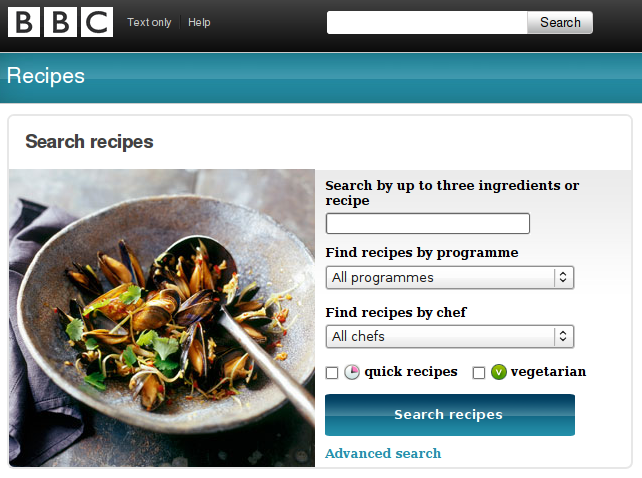
\includegraphics[width=0.9\textwidth]{screenshot_bbc_recipes}
\caption{The BBC Food Recipe Search Page}
\label{fig:bbc_food}
\end{figure}

The aim of this project is to develop a software kitchen assistant tool. This tool must be able to provide recipes which match a supplied list of available ingredients. This is similar to the BBC's recipe search\footnote{\url{http://www.bbc.co.uk/food/recipes/}} (Fig~\ref{fig:bbc_food}), but is not constrained to just three search items. The software should, in essence, provide recipe matches to help the user make recipe decisions given the ingredients he/she currently has. This involves making recommendations and provides us with an avenue to make use of collaborative filtering technology. Additionally, the recipe database can be community maintained, and aspects of social networking can be implemented to encourage user participation. The main draw of the project lies in its inherent flexibility, which extends from the plethora of expansion decisions which can be made to enhance user experience.

\newpage

\section{Expanded Problem Description}
As a group we understood that the aim of the project is to develop a software kitchen assistant tool. The tool must be able to provide recipes which match a supplied list of available ingredients. The software should provide a number of matching recipes and rank the suggestions according to how well they match. The database will also take into account user’s own food preferences, this allows us to introduce collaborative filtering technology to manage the recommendations. 

We have chosen to use extreme programming therefore making frequent and small releases. We have specified three versions, these being minimum, realistic and ideal. 

For all three versions the interface of the kitchen assistant tool will be web-based and will allow the user to select at the least three ingredients. Once these ingredients are submitted it will return a list of recipes that are ranked in accordance to how well the recipe matches the selected ingredients. 

Version 1 will be a web-based application with a simple interface using only HTML, CSS and Django template markup. The online database will contain several recipes that are searchable by ingredients.

Version 2 is an extended version of v1.  The web-based interface will introduce JavaScript, AJAX (asynchronous JavaScript and XML) and JSON (JavaScript Object Notation). The online database for this version will contain a vast amount of recipes that are searchable by a combination of ingredients. With the introduction of collaborative filtering we intend to create user accounts that allows the user to rate recipes and then return recommendations based on previous ratings. 

Version 3 extends v2. The web-based interface will remain the same however we will create a mobile optimised interface and an Iphone application. The online database for this version will include a very large amount of recipes that are automatically updated and maintained. Recipes will be searchable by combinations of ingredients and by other tags such as ‘vegetarian’, ‘Italian’, ‘low fat’, etc. Returned recipes will be returned based on past ratings and accumulated data from the entire database. Recipes will also give recommendations for several users i.e. ‘A recipe that alice and bob will both like’. This version will include a full user system with profiles and user-uploaded recipes. The application will support social media functions such as messenger, the possibility of rating, tagging and commenting on other recipes. 

The project has be divided into 5 managerial area’s. These being management, technical, design, quality assurance and documentation. Every member has been given the responsibility of one of these areas and is expected to ensure all targets are met.



\newpage

\section{Research} %quite aware this is in the wrong place, idk where the right place is. please rearange the following
\subsection{BBC Recipes}

\begin{figure}
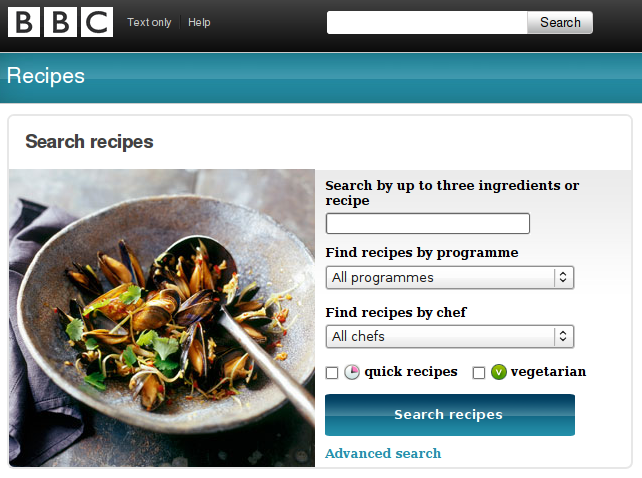
\includegraphics[width=0.9\textwidth]{screenshot_bbc_recipes}
\caption{The BBC Food Recipe Search Page}
\label{fig:bbc_food}
\end{figure}


BBC Recipes (Fig~\ref{fig:bbc_food}) is a web application that allows the user to input up to three ingredients and returns a list of related recipes. 

BBC Recipes has two search options, basic and advanced. The basic search allows the user to input up to three ingredients with the option to find the recipe by television program or by chef. This search also provides the tagging options of quick recipes and vegetarian. However the advanced recipe search includes a wider choice of search preferences such as, the preparation method, cuisine, season and dietary requirements. After looking over the source code it’s very obvious that this web-based application uses an online database using a query language to return recipe results. 

One main advantage about this application is the advanced search option which includes a numerous amount of tag options. This option becomes quite useful when searching through a large database as this kind of search minimizes the results. A good example of this is a search including flour, butter and sugar with the season tag being ‘Christmas’ and the dietary needs tag being ‘nut-free’ returning only 14 recipes. However a search including just the three ingredients returns 400 recipes. 

One flaw that I have noticed with the search is that the search field is a text box which involves text input, this not validating the input until creating the search. The validation matches the input with similar words, for example for ‘flor’ it will return ‘flour’. However when having typo’s like ‘aooples’, instead of ‘apples’ the returned match is ‘allows’. To solve this issue a drop-down menu including the ingredients from the database would perhaps be a better idea.

The design of the website is attractive with a good use of colour and images. However the navigation of the website is slightly tedious, the reason for this being when expanding the actual recipes on the home page the webpage’s content increases and therefore leaving the user to have to scroll through the webpage to view it’s content. 



\subsection{RecipeZaar.com}

\begin{figure}
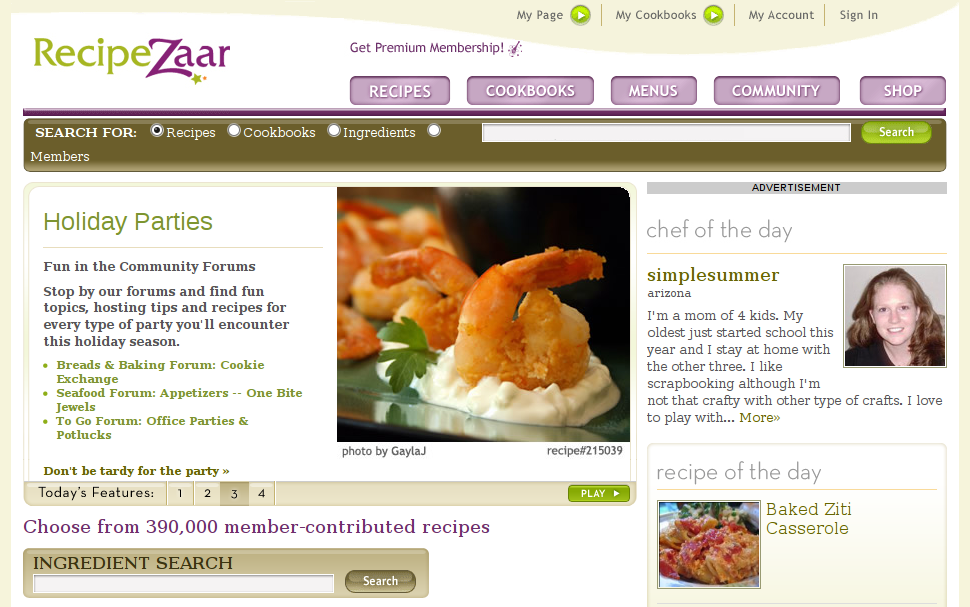
\includegraphics[width=0.9\textwidth]{screenshot_recipezaar}
\caption{The RecipeZaar.com Home Page}
\label{fig:recipezaar}
\end{figure}

Recipezaar (Fig~\ref{fig:recipezaar}) is a website that includes a large database of recipes and user accounts. Recipes are searchable by recipes, cookbooks, ingredients and members. 

The recipe search allows the user to input n number of ingredients. The input method is a text box which includes no validation. If the user inputs ‘flor’ instead of ‘flour’ the search returns nothing. The query used for this search seems to be very basic, the reason for this being if the user inputs ‘flour, sugar, butter, eggs’ for example one of the returned recipes is ‘vegetable casserole’ which doesn’t contain any of the above ingredients. Another example of a recipe is ‘leach family turkey stuffing’ which only contains one of the above ingredients. Because the search isn’t specific and because the website has a large online database the results are too vague.

This website introduces the use of collaborative filtering by including user accounts with the option to upload recipes and rate other recipes. When viewing a member’s recipe theres also the option to send a private message, submit corrections, send the recipe to the users email address or mobile device and create a shopping list. The recipe page also directs the user to other recipes ‘like’ the chosen recipe. The website also has a community webpage with forums for general discussions. 

The design of the website is interactive with a good use of JavaScript. The colour scheme is neutral with a good use of images.




\newpage

\section{Results of Technical Research}		%new section on research

For this part of the project we looked into many different alternatives for suitable platforms,
tools, technologies, algorithms and data structures. We mainly conducted our research using the internet however, 
we did use some of our own personal experience and preferences aswell to influence our decisions.

\subsection{Platform Decisions}

\paragraph{Microsoft Windows}
The windows operating systems have long dominated the operating system industry. Approximately 90 \% of users use Windows operating systems, chiefly Windows XP followed by Windows Vista. Its ease of use and engaging graphical interface is certainly an attraction. However, precisely due to its widespread usage, Windows is the prime target for malware. Microsoft however, does provide bug fixes and other help to stabalise the system. Moreover, most forms of software run on Windows.

If our group is to market our product to customers, it makes sense that we focus on Windows as the platform of choice since it is the most commonly used operating system. Moreover, if our project decides to make an application, it should be able to run in Windows, and since most software works on Windows, it is the clear choice.

\paragraph{Mac OSX}
Although not as widely used as Windows, this operating system has a very encouraging user interface which is easy to pick up. It is claimed as being more secure than Windows, due to its UNIX base. However, recent reports suggest the Apple’s Snow Leopard system is less secure compared to Windows Vista and XP\footnote{ [ http://www.wired.com/gadgetlab/2009/09/security-snow-leopard/ ].}. Of course we must take into account the comparatively fewer threats from malware on Mac OSX. 
Mac OSX also uses pre-emptive multitasking for all native applications to which decreases the incidence of multiple program crashes.

\paragraph{Linux}
One of the biggest advantages of Linux over other operating systems is the Linux kernel which ensures a basic level of security. Its hardware requirements are also much lesser than Windows and Mac OSX. Additionally, Linux, being open source is a free system. Linux distributions like Ubuntu, also provide a friendly and graphical user interface for users to work with. However, latest hardware is typically slower to reach linux. Moreover, depending on the distribution, the learning curve of Linux might be daunting for users \footnote{[ http://packratstudios.com/index.php/2008/04/06/the-pros-and-cons-of-linux-windows-and-osx/ ]}.

\subsection{Technologies}

\paragraph{Django}
A web framework based on Python language, Django is relatively easy to understand, Python being easier to program due to its natural language-like syntax. One of chief arguments for the use of Django concerned software reuse. Various existing libraries can be used to aid our software development efforts. The group software head also backed Django, and his recommendation was well received since the group could learn a new form of technology while benefiting from his expertise.
\begin{itemize}
\item Advantages
	\begin{itemize}
	\item Our Technical Officer has experience developing with Django which is beneficial when developing and learning the language.
	\item Python is an easy language to learn and use, with a focus on simplicity and ease of use whilst providing an elegant solution to the problem.
	\item A variety of third party plugins coincide with our site's functionality, saving a lot of work by maximising code reuse.
	\end{itemize}
\item Disadvantages
	\begin{itemize}
	\item Requires learning a new language.
	\end{itemize}
\end{itemize}


\paragraph{Ruby on Rails}
A web framework based on Ruby language, it allows users to create powerful applications using simple coding without compromising on the functionality of powerful languages\footnote{[ http://www.hosting.com/support/rubyonrails/faq/ ]}. The Rails framework also has many pre-defined libraries and functions that we may be able to use to our advantage.
\begin{itemize}
\item Advantages
	\begin{itemize}
	\item Increased code reuse due to vast array of pre-defined libraries and functions available.
	\item Also provides an esay and elegant solution to complex web programming problems.
	\end {itemize}
\item Disadvantages
	\begin{itemize}
	\item Abstraction may mean sacrificing fine control even when it would be useful.
	\item None of our group are familiar with the Ruby framework which may affect our pre-defined timetable and/or our time constraints.
	\end {itemize}
\end {itemize}

\paragraph{PHP with SQL}
This option was an attractive one, considering that members had some experience with PHP and SQL previously. Moreover Java, Python, C++, Ruby are normally used to create complex systems which is not necessary for us 
at this stage in the project.
\begin{itemize}
\item Advantages
	\begin{itemize}
	\item Overall group experience with these languages. 
	\item Common technology means it is well supported with many tutorials and guides on usage.
	\end {itemize}
\item Disadvantages
	\begin{itemize}
	\item Low level control means making large systems is complicated and difficult.
	\end {itemize}
\end {itemize}

\paragraph{Web Browser Options}
In theory, all web browsers are the same, and any page that works on one will work on all others, as long as they all support the same standards. In practice this is not the case and different browsers support different features. The main browsers right now are Microsoft Internet Explorer, Mozilla Firefox, Safari, Google Chrome and Opera\footnote{\url{http://www.w3schools.com/browsers/browsers_stats.asp}}. Of these, the majority support the web standards codified by the World Wide Web Consortium (W3C)\footnote{\url{http;//www.w3.org}}, so in order to easily gain compatibility with the largest number of web browsers, we will aim to write a W3C standard compliant site. We can test this with W3C's validator\footnote{\url{http://validator.w3.org/}}, which will save us having to debug the site in every browser we wish to support






























\newpage

\section{Collaborative Filtering Technology}
The final prototype of our project deals with users being able to rate recipes and receive recommendation of recipes they might like. There are a number of ways this system can be implemented with collaborative filtering technology. Collaborative filtering technology provides numerous prediction algorithms which we can use to implement such a system and acquire ratings.

\subsection{About}

Collaborative filtering (CF) is the process of evaluating items through the opinions of other people \footnote{r  Schafer J.B., Frankowski D., Herlocker J., Sen S.: Collaborative Filtering Recommender Sytems}. While the concept of collaboration is nothing new or novel- it is in human nature to take the opinions of other people- the technology itself was developed in the early 90s[r]. The main difference between collaboration in everyday life and through the internet is that the internet allows us to utilise the opinion of large communities. 

One of the earliest systems utilising the collaborative approach was Tapestry, developed by Xerox Parc\footnote{Goldberg D., Nichols D.,Oki B.M.,Terry D.: Using Collaborate Filtering To Weave An Information Tapestry. Communiation of the ACM, 35(12): pp 61-70}. Tapestry stored textual information, along with metadata and annotations about this information upon, which users could apply queries.

Users are recommended items based on their ratings for particular items. There are two ways a rating may be acquired- either explicitly or implicitly. Ratings are gathered explicitly when the user submits an opinion on an item, as opposed to implicit ratings which are inferred from user actions[].

Collaborative filtering is especially relevant to our project since it addresses the user task of helping users find recipes that he/she might like. The functionality we would like our system to have is that of constrained recommendation, as opposed to dealing with prediction (where given a particular recipe, calculate its predicted rating). Constrained recommendation is suited to our project because it allows users to input particular constraints, in this case, the recipe ingredients, and from the list of recipes generated, recommend users the recipe [ ]. Provided the numerous number of recipes in the database, and given a users limited attention span, it would be logical to return a recommendation which the user is more likely to appreciate.

\subsection{System Pre-requisites}

However, this technology will work effectively provided the domain it is applied to meets certain criteria. In our case, 

\begin{enumerate}
\item	The database should hold many recipes 
If too few recipes then there is no point of recommendations.

\item	There must be many ratings for a recipe
For a useful recommendation, the recipe needs enough ratings. Assuming each user rates only few recipes, and the large database of recipes, this implies that there must be a sufficiently large amount of users.

\item	Users must rate multiple recipes
Else, we will be unable to relate recipes to each other.

\end{enumerate}

\subsection{Algorithms}

Algorithms can either be probabilistic or non-probabilistic. Probabilistic algorithms use probability distributions to compute, for example ranked recommendation lists. However, non-probabilistic algorithms models are more popular with practitioners[]. 

\subsection{Non-Probabilistic algorithms}

\subsubsection{User-based Nearest Neighbour Algorithms}

Predictions are generated here for users based on ratings from similar users, called neighbours. By analysing all the users neighbours, a rating can be predicted for a particular item for the user. Neighbours who are more similar to the user will have a higher weight in calculating the rating. Such similarity is elucidated by the Pearson correlation. Additionally, a neighbours personality will be adjusted for (some may be optimistic and rate consistently high and pessimistic neighbours rate consistently low even if both neighbours mean the same thing). 

However, there are many caveats with this algorithm. If there are few ratings, then the matching of a users and a neighbours ratings will be biased, such that a particular neighbour will start heavily influencing the users neighbourhood. Additionally, the formula for this algorithm does not account for popular items. If numerous people agree that a particular recipe is excellent, then this data is less important than one in which users agree on a recipe of debatable taste. Moreover, basic implementations of this algorithm have linear time and memory requirements[]. Although, there are techniques which help alleviate such requirements (e.g. clustering) they also have their own limitations.

\subsubsection{Item-based Nearest Neighbour Algorithms}

 Conceptually similar to user-based nearest neighbour algorithms, this algorithm focuses on acquiring ratings based on similarities between items. Adjusted-cosine similarity is the most popular and accurate [] way to calculate similarity between items. It is very similar to the Pearson correlation that is used with user-based nearest neighbour algorithm. There exists reports which suggest that item-based nearest neighbour algorithms give more accurate predictions compared to user-based\footnote{r52Sarwar B., Karypis G., Konstan J.A., Riedl J.:Item-based Collaborative Filtering Recommendation Algorithms. Proceedings of the 10th international conference on World Wide Web. (2001) Hong Kong. ACM Press p.285-295}.

A big disadvantage is the complexity of the algorithm, whose size could be the square of the number of items, although, there exists ways to prune the size of the model [sarwar only k coratings]. However, pruning causes difficulty prediction. Additionally, items cannot have too few ratings as this may lead one item to heavily influence a prediction.

\subsubsection{Dimensionality Reduction Algorithms}

These algorithms help reduce the complexity of very large systems with a lot of items. They map the item space to underlying tastes of the user, which diminishes the system runtime complexity. Typically, a vector based technique like vector decomposition[] can be used to extract these tastes. This way, a prediction can be found reasonably.

However, techniques like vector decomposition require complex mathematical computation to produce the taste-space. Although heuristic methods help in updating this taste-space to avoid constant recalculation, software maintenance is hard due to this complexity. Reportedly this reduction in complexity is not a significant enough improvement.

\subsection{Probabilistic Algorithms}

Probabilistic algorithms employ well established concepts of probability to make predictions. Baynesian-network provide the preferred framework to generate reliance among users or items[] and can be implemented as decision trees to represent probability tables [9, diagram] for example. 
Expectation maximisation algorithm [hoffman,29] also uses Gaussian probability distributions to extract user underlying tastes.

One advantage of these algorithms is that not only can they help calculate the most probable rating but they also help compute the plausibility of the rating.

\subsection{General concerns about all algorithms}

If there are too few ratings then none of the algorithms will yield any useful data due to biasness. There are a number of techniques that help mitigate such problems. For example you can choose to discard items with ratings which are below a certain number although, this will reduce the scope of the collaborative filtering system.

\subsection{Acquiring Ratings- Design Decision}

There are two way to collect ratings- explicit and implicit. Explicit ratings are usually more accurate description of the users preferences however, this requires some input from the users end. It was previously believed that the users would rarely choose to spend their time rating an item, however, experience has refuted this belief as exemplified by websites such as Youtube[]. Moreover, incentives can be used to entice users into rating, for example, reward points.

In contrast, implicit ratings require no input from the user but they usually are not as accurate as explicit means. For example, the amount of time the user spends reading a recipe might be an implicit mean of ratings collection (the more time the user spends reading the recipe, the more he/she will likely like the recipe), but this may be inaccurate as the user may not like the recipe after reading it. However this uncertainty will be assuaged if you are able to collect a large amount of such implicit data. 

\subsection{Rating Scales }

Another issue is selecting rating scales. If you provide a rating scale with more options, it will provide more information about the user. That is not to say that you provide a rating scale with an unnecessarily large amount of options, which may not add value to the system. Importantly, you must consider the needs of the users. If you provide too few ratings on the scale, users may find that they cannot express their opinions accurately. 

\subsection{Cold Start Issues}

These issues refer to when the system is unable to provide a useful recommendation to the user due to an initial dearth of ratings. This can occur as the following scenarios:

\subsubsection{New User}
No specific predictions can be made to the new user since he/she has not made any ratings yet. This can be overcome, for example, by asking the user to rate some initial items before they can register the service or by obtaining demographic information from the user and matching his/her ratings with other users of similar demography.

\subsubsection{New Item }
The new item will initially have no ratings so it will not be recommended. This can be overcome by recommending items through non-CF techniques like content analysis \footnote{r53 Sarwar B., Karypis G., Konstan J.A., Riedl J.:Incremental SVD-Based Alogorithms for Highly Scaleable Recommender Systems. Proceedings of the Fifth International Conference on Computer and Information Technology (2002)} or random selection of new items and asking for ratings on those items.

\subsubsection{New Community}
If there are no ratings then the system cannot provide recommendations to users who seek this service. User retention will diminish. A solution is to provide rating incentives to a small subset of the community[], before expanding the service to the entire community. 

\subsection{Challenges with Collaborative Filtering}

The obvious challenge is that of privacy. For a system provide accurate recommendations, it is necessary as much information about the user as possible. However, if a user divulges too much information, he/she is at risk if the central database containing this information is compromised. Additionally, the user should trust the particular website to not misuse user information.

Another issue is of trust. Users can purposely give artificial ratings which are not representative of their true opinions. Companies can manipulate recommender systems as well by overwhelming the system with favourable ratings of its own products \footnote{[6 BBC News Online, ``Sony Admits Using Fake Reviewer.'' June 4, 2001 \url{https://news.bbc.co.uk/1/hi/entertainment/film/1368666.stm}]}.

\newpage

\section{Product Specification} 			%Product Spec
\label{sec:productspec}
In response to our initial meeting with our client and after reviewing the ''Problem Description'', we have put together a brief specification stating the requirements for the software at three levels which have been agreed by our client. The levels can be considered as versions as they will be implemented in this way (i.e. Minimum - version 1.0, Realistic Best -  version 2.0 and Ideal - version3.0 \footnote{It should be noted that due to the nature of creating a solution there are likely to be intermediate versions e.g. 1.2, which will be used solely in the repository.}). These requirements will be used as a basis for the design of the respective versions and the designs will be created with these requirements in mind.

\subsection{Minimum - v1.0}

The requirements listed below are the minimum requirements to make the software work which does not include extra functionality desired by our client. This will be the Version 1.0 of our prototype and we will use this as a base to build from. 
Furthermore, the creation of different versions with the intent to expand on previous versions will allow for continuity between languages and eliminating the need to 'start from scratch'.

\begin{itemize}
	\item Contains several recipes in a database.
	\item Has a Web Interface.
	\item Recipes are searchable by ingredients (greater than 3 ingredients).

\end{itemize}

\subsection{Realistic Best - v2.0}

The requirements below are what we have identified as the most realistic outcome of the software within the time constraints. This would meet all the minimum requirements outlined by the client and some desirable ones as well. This will
essentially be an expanded/upgraded version 1.0 .

\begin{itemize}
	\item Has a large database of recipes.
	\item Has a clean, attractive web interface.
	\item Has a seperate, simpler web interface for mobile devices.
	\item Recipes are searchable by combinations of ingredients.
	\item Has user accounts.
	\item Allows users to rate recipes.
	\item Gives recipe recommendations based on past ratings.
\end{itemize}

\subsection{Ideal - v3.0}

Below are the requirements for the software if it were to be the ideal solution to the problem. This list includes existing requirements from v1.0 and v2.0 at a higher level and all desirable requirements as well. It is likely that only few of these requirements will be fulfilled in the final version that is submitted. 

\begin{itemize}
	\item Has a very large, automatically updated and maintained database of recipes.
	\item Has a clean, attractive and user-friendly web interface.
	\item Has a mobile device optimised interface and an iPhone application.
	\item Recipes are searchable by combinations of ingredients.
	\item Recipes are searchable by other tags: 'vegetarian', 'italian', 'low fat' etc.
	\item Has a full user system with profiles and user-uploaded recipes.
	\item Supports social media functions.
	\item Allows users to rate, tag and commment on recipes.
	\item Gives recipe recommendations based on past ratings and accumulated data from the entire user base.
	\item Gives recipe recommendations for several users i.e. 'A recipe that Alice and Bob both like'.

\end{itemize}

\newpage

\section{Initial design of the proposed system and its user interface}
The version 1 website colour scheme is an amalgamation of white (for the background) and orange (for miscellaneous design features). The white background leverages on its simplicity and clarity, an important criteria for retaining the attention of the user. Moreover, the orange colour is reportedly stimulating for the users appetite\footnote{[ http://desktoppub.about.com/cs/colorselection/p/orange.htm ]}. The group also agreed on an orange logo design. 

\subsection{Version 1}

\begin{figure}[h]
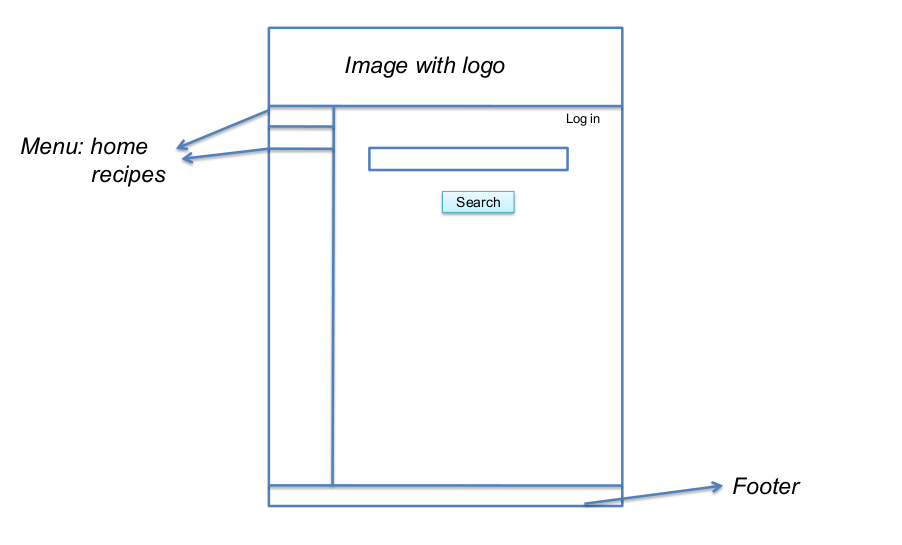
\includegraphics[width=0.9\textwidth]{home_page}
\caption{Layout of the Home Page}
\label{fig:home_page}
\end{figure}

The merit of the version 1 website design is in its simplicity. Upon accessing the website, (Fig~\ref{fig:home_page}) users are presented there are three drop-down menus which allows people to select ingredients. The drop-down menus are transversely positioned to accommodate the vertical cascading of the ingredients of the menus. Users are provided with three menus to select ingredients and submit a search. This then links to the recipe list page. Additionally, the “recipes” button in the sidebar links the page to the complete list of recipes alphabetically.

\begin{figure}[H] % Place it [H]ere, you big furry oaf! I don't care what you smell! 
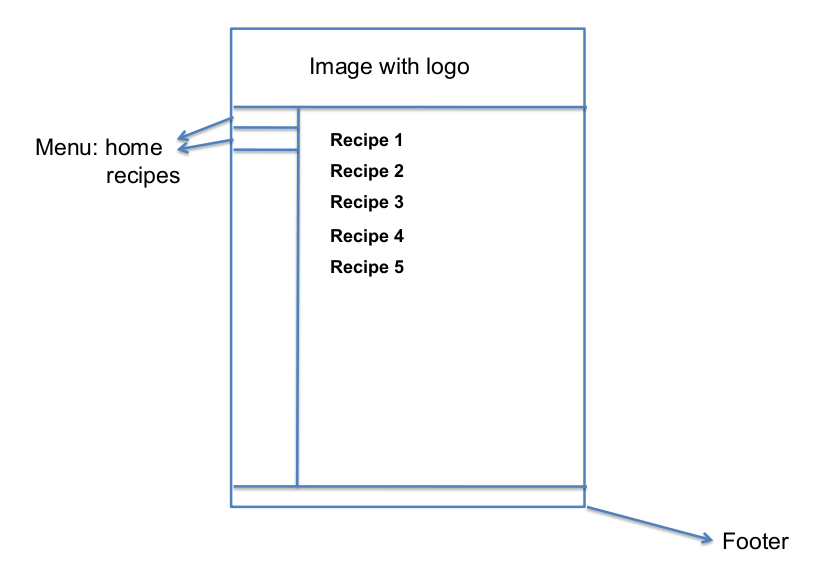
\includegraphics[width=0.9\textwidth]{recipe_list_page}
\caption{Layout of the Recipe List Page}
\label{fig:recipe_list}
\end{figure}

The recipe list page (Fig~\ref{fig:recipe_list}) contains a list of recipes with at least one of the three ingredients. However, the recipe may contain other ingredients which were not specified by the user. Upon recipe selection, the specific recipe page will be displayed.

\begin{figure}[H]
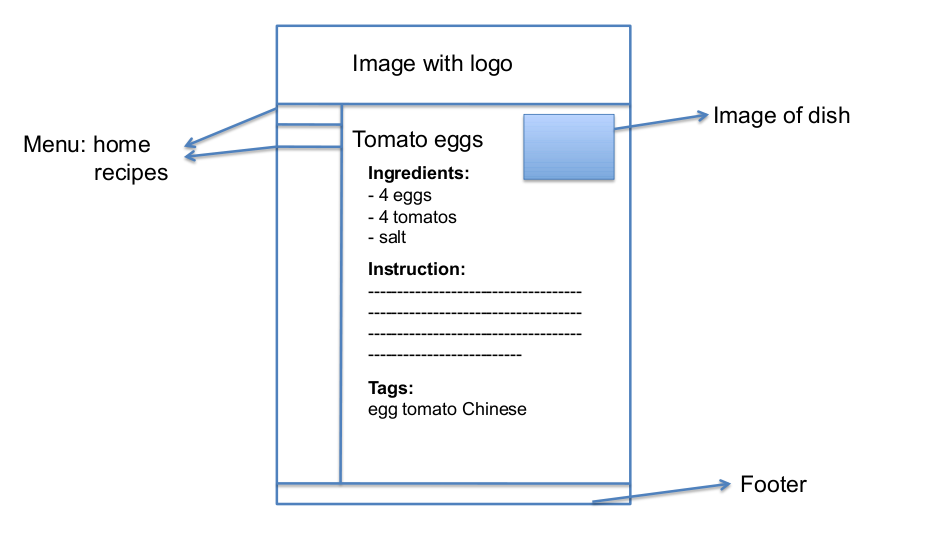
\includegraphics[width=0.9\textwidth]{recipe_page}
\caption{Layout of the Recipe Page}
\label{fig:recipe_page}
\end{figure}

The recipe page (Fig \ref{fig:recipe_page}) contains recipe details, for example recipe name, ingredients, the instruction, and recipe tags.
 
One design limitation of version 1 is that the website only has three drop-down menus, and the user is unable to type in ingredients. Being a prototype, the version 1 database is fitted with few recipes hence such functionality is redundant. 

\subsection{Version 2}
Version 2 is an upgraded version of the original version containing more functions (described by the Product Specification). With the use of technology such as JAVA Script, the web interface will look more polished. Users will be able to enter text data into ingredient selection text boxes, which will have the tab completion feature for ingredients instead of using a drop-down menu. There will also be a larger database of ingredients hence justifying the use of tab completion as apposed to drop-down menus.

Additionally, for version 2, users are allowed to have web accounts. The benefits of the account include the user having access to past recipes which he/she rated and more importantly receive recommendations of recipes they might like (this uses collaborative filtering technology). In addition, users could choose to click tags and get a list of recipes that contains that particular tag.

Additional website link may likely be created, for example a link to the most popular recipes. The website is also expected to be optimised for mobile phone viewing.

\subsection{Version 3}
The ideal version of our product involves the implementation of a variety of possible functionalities. For example, a mobile application could be developed. Recipes could be made searchable by not just ingredients but also, for instance, the type of cuisine (Chinese dish) or whether recipes are vegetarian or non-vegetarian. 

Social networking is another possibility, with users being able to interact with other users and leave comments of the pages of other users. Users might be able to upload their own recipes and receive ratings from other users. The possibility for improvements are abundant.

\newpage

\section{Implementation Options/Designs}
\subsection{Summary of Project Description and Specification}

The project description implies the implementation of some form of a database, either online (i.e. on a website) or offline (i.e. run on a local machine as an executable program). There are no specific details as to which language, layout or structure etc, are to be used when creating the solution. There are also no details as to which Operating System the solution should be created for and whether additional software/hardware is allowed. Considering this we have ‘taken it open ourselves’ to discuss and choose what we thought was a suitable target platform and have also discussed availability of software/hardware needed to create the solution.
During an initial meeting with our client concerning the problem specification/requirements it has become clear that the preferred solution is to create a website with a database backbone. This can be implemented in many different styles/languages which we have also discussed extensively.
 
We have created the Problem Specification (section~\ref{sec:productspec} on page~\pageref{sec:productspec})
% You can stick labels to sections and have it update the page number if it changes!
 with the intent that at each stage, the structure and format of the solution allows successive stages to be completed without changing the entire structure too much. This prototyping adheres to a large extent with the concept of Extreme Programming, where frequent releases introduce checkpoints where new customer requirements can be adopted. Additionally, the focus will be on upgrading versions of prototypes. To accommodate this dynamic character of our project, we need a framework which ties in the database with all the different elements of the website.


\newpage

\section{Implementation Decisions}

\subsection{Decision Influences}

\subsubsection{Aims}

The aims of version 1 have a strong influence over implementation decisions. They are as follows;

\begin{enumerate}
\item To be a complete working release of a usable piece of software
\item To allow the team to familiarise themselves with the tools and systems to be used for later versions
\item To explore the capabilities of those systems, to inform and inspire later decisions.
\end{enumerate}


\subsubsection{Design Principles}

The project is being developed using a version of the Extreme Programming (XP) Methodology. XP's software development principles have an impact on the software design principles of projects developed using it.

Similarly the Web Framework Django has its own set of design philosophies\footnote{\url{http://docs.djangoproject.com/en/dev/misc/design-philosophies/}} which also influence the project's design principles.

The principles of XP and Django are quite similar and complement one another quite well, so it is possible to abide by both sets of principles without contradictions.

Some of the XP/Django principles that have the most influence on implementation decisions are listed below;

\begin{description}
\item[DRY] Don't Repeat Yourself \\
Every piece of knowledge must have a single, unambiguous, authoritative representation within a system.
\item[YAGNI] You Aren't Gonna Need It \\
Always implement things when you \textit{actually} need them, never when you just \textit{foresee} that you need them
\item[Maximise Code Reuse] If two bits of code look similar, move them out into a more general function. If two functions do a similar thing, merge them. This keeps redundancy low.
\end{description}

Both XP and Django have a strong basis in philosophy and principles, and while they both leave the developer the freedom to chose their implementation decisions, they are designed to work best with implementations that follow their principles.

\subsection{Decisions}

\subsubsection{The \texttt{recipes} App}

Recipes are the only thing that version 1 does, so it would make some sense to simply have the project as a whole perform the recipe functions, and not use any apps. However, the functionality of the site was put in a \texttt{recipes} app for two reasons.
Firstly, it is best practice in Django to have all code in conceptually distinct, reusable apps, to maximise potential code reuse.
Secondly, as one of the aims of this version is to introduce the team to working with Django, and apps are a major part of Django, it made sense to use apps even if they are not strictly necessary.


\subsubsection{URL Design}

The URL design is intended to be very simple and readable. In accordance with Django URL design principles, there are no filename extensions in URLs.


\subsubsection{Model Design}

The only implementation decision of note in the model design is the use of a python \texttt{property} to handle recipe tags. A \texttt{property} is a python language construct that behaves as though it is a class variable, but behind the scenes calls a getter or setter function when it is fetched or assigned to. This was used because, although it makes the model less readable, it makes all of the code that deals with the model far more readable, and it is this code which is more complex and benefits more from simplification.

\subsubsection{View Design}

\paragraph{The \texttt{recipe\_list} View}

There are 2 views that simply show a list of recipes:- \texttt{recipes\_all} (the view of all recipes on the system) and the results section of \texttt{search} (the view of all recipes that meet the search terms). In order to maximise code reuse, the functionality of displaying a list of recipes was taken out into a separate \texttt{recipe\_list} view, which is called by both \texttt{recipes\_all} and \texttt{search}.

\paragraph{The \texttt{search} View}

The search is deliberately the simplest search possible that meets the specifications. The set of results is simply the set of recipes which contain any of the ingredients searched for. This will be radically improved in later releases.

\subsubsection{Template Design}

\begin{samepage}
\begin{quote}
``The most powerful -- and thus the most complex -- part of Django's template engine is template inheritance. Template inheritance allows you to build a base ``skeleton" template that contains all the common elements of your site and defines blocks that child templates can override."\flushright-- Django's Template Documentation\footnote{\url{http://docs.djangoproject.com/en/dev/topics/templates/}}
\end{quote}
\end{samepage}

\noindent Template Inheritance provides a good opportunity to maximise code reuse, but it was not used in version 1 in an attempt to keep template design simple.














\newpage


\section{Implementation Results}
Version 1 largely adheres to the design specification.

\begin{figure}
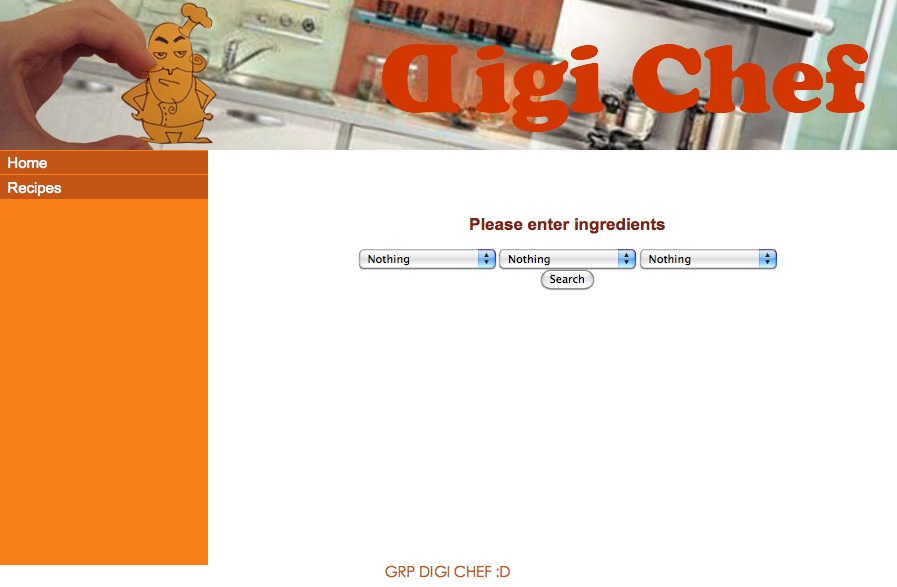
\includegraphics[width=0.9\textwidth]{result_1}
\caption{Homepage}
\label{fig:result_1}
\end{figure}


As mentioned, white and orange are the colours of choice, along with an appealing logo. The design is simple and effective in meeting the needs of version 1.(Fig~\ref{fig:result_1}) shows the drop down menus for ingredient selection with the search option.

(Fig~\ref{fig:result_2}) shows the result of ingredient selection by the user. The recipe list was generated based on the ingredients selected by the user.

\begin{figure}
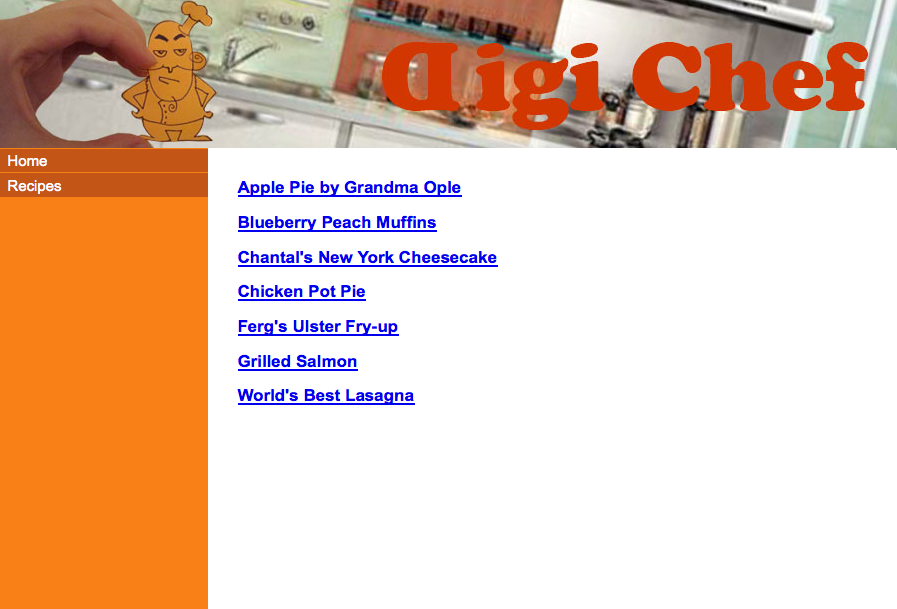
\includegraphics[width=0.9\textwidth]{result_2}
\caption{Search results}
\label{fig:result_2}
\end{figure}

(Fig~\ref{fig:result_3}) shows the result of clicking on a recipe. Notice the Recipes button on the far left hand side of the web page. Clicking that generates the list of all recipes in the database.

\begin{figure}
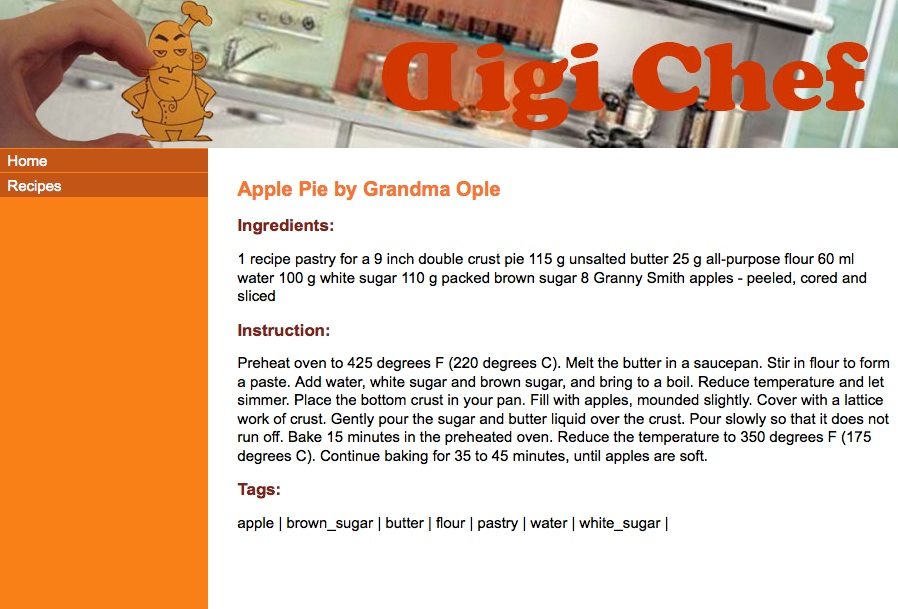
\includegraphics[width=0.9\textwidth]{result_3}
\caption{Recipe page}
\label{fig:result_3}
\end{figure}

The group thoroughly scoured the website of bugs by doing exhaustive testing of all the possible ingredients and checking if the returned list matches the input ingredients. Exhaustive testing was possible for version 1 due to the small database and only three ingredient boxes. However, as our system gets more complicated, this form of testing will be unwieldy. A better method of testing will be required then.


\subsection{Implementation Points of Interest}

\subsubsection{Collaborative filtering implementation}

The implementations of collaborative filtering methods in the module \texttt{django-recommender} were not as suitable for our needs as they first appeared, and had to be modified.

Some of these modifications were simple, for example there was no easy way to search for a recipe based on a set of tags, which we needed to implement search. A new method was adapted from an existing method which found items similar to a given item. The original method used the tags of the given object to do the similarity comparison, so the new method skipped the stage of extracting the tags from the given object and had the tag list be passed in as an argument in place of the object.

Others were more difficult. The method designed to recommend recipes to users was designed to work on tagged users. The idea here was that users would tag themselves with things they like. For example in a film rating system, action fans would tag themselves with `action', the same `action' tag applied to action movies. In this context that made little sense, as people are rarely `fans' of individual ingredients, and no-one is going to want to tag themselves `onion'. So I wrote my own rating prediction function based on the equations in the collaborative filtering research section of the report, from scratch.

The method I used was the final user-based nearest neighbour method in the research:

\begin{equation}\label{eq:avgadjust}
pred(u,i) = \overline {r}_u + \frac{\sum_{n\subset neighbours(u)} userSim(u,n)~\cdot~(r_{ni}-\overline {r}_n)}{\sum_{n\subset 
neighbours(u)}userSim(u,n)}
\end{equation}

A direct translation of this function into code was implemented. This proved to be extremely inefficient, taking approximately 1.5 to 2.0 seconds to rate each recipe, suggesting a total recommendation time for the database of 24 to 31 minutes. This was obviously unacceptable, so optimisations were sought.

A lot of things were being unnecessarily recalculated each time. Some of these things, like average vote for a user, or a 1-dimensional array of all votes for a user, could be calculated once per vote and stored in the database, so these calculations were moved to the voting part of the operation. This introduced a small delay in voting, which is far less of a problem than it would be here, because voting is done with \textsc{Ajax}, so the user isn't interrupted, and voting is very fast anyway. These re-factorings made the method run on one tenth the original time.

Some things, like the sum of similarity ratings to neighbours, had to be calculated each time recommendations were sought, but not for each recipe, so these were moved to be pre-calculated before the loop over recipes. Moving out the similarity sum calculations doubled the running speed again, and pre-calculating individual user similarities caused further drastic speed increases. The final implementation operated 171 times faster than the original.



\newpage


\section{Summary of General Problems Encountered}
The project required that members familiarise themselves with forms of technology that they were unfamiliar with, for example Django (a python web framework). Learning such software required extensive learning from web tutorials and other sources like books. Naturally, most of the technical difficulties concerned Django. For example, it took a significant amount of time to learn about how to process forms using Django. When users select an ingredient from the drop down menu, knowledge of Django forms was essential in retrieving relevant information from the database about the recipe. 

Additionally, members were required to learn new concepts like collaborative filtering and extreme programming. This was namely done by immersing in web research and group discussion. The Project Supervisor also helped in the clarification of key concepts by delivering a series of discussions during formal meetings.

The team has a clear management structure which has prevented any issues. Moreover, this enables members to take responsibility of their areas, thereby ensuring accountability and alleviating conflicts. This also ensures an equitable distribution of workload.




\section{Conclusion}
The success of version 1 of our protype within the set deadlines is a testament to the group's
dedication to the project. This achievement also provides valuable affirmation to having set a reasonable timeplan and project 
specification.

Version 2 was met before the deadline, and there was time to implement a few extra features from the ``Ideal System'' Version 3 specification. Although it was a very challenging specification, the group had ambitious plans for further developments that could be made, and the structure of the project is designed to be extensible to allow such future features to be implemented. The project already surpasses many commercial services in its more advanced features, and with more development time we believe that it could lead the field.

\newpage



\section{Appendices}
\subsection{Timescale}

\begin{figure}[h]
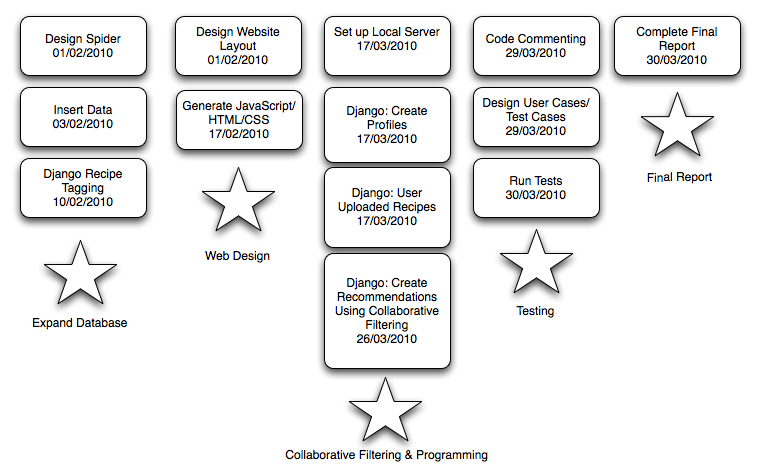
\includegraphics[width=0.9\textwidth]{milestone}
\caption{Project Timescale}
\label{fig:milestone}
\end{figure}

The project timeline can be decomposed to 4 key deadlines:
\begin{enumerate}
	\item Interim report submission (04/12/2009)
	\item Final report due (01/04/2010)
	\item Open day (05/05/2010)
	\item Presentation day (07/05/2010)

\end{enumerate}



Since our group is adopting the methodology of prototyping, a milestone chart is to be made for each of the three versions which conform to the above deadlines. Above is the detailed timeline of the version 1 prototype expressed as a project milestone chart (Fig~\ref{fig:milestone}).
Each oval represents a downward progression to the milestones, represented by stars. The dates represent the deadlines that the group deemed appropriate for each progression. The group decided early on to plan out the web and database design together, which is essentially “the meat” of our project. Thereafter, tasks will be allocated to each member where the individual heads of the project will take charge of their respective domains. Deadlines of specific tasks are as elucidated by the above. Notice that version 1 is to be completed before the deadline for the interim report which exemplifies the fact that our chart takes into account the major deadline dates.

Due to the dynamic nature of our project, it was decided that further milestone charts will be designed as we progress from the completion of one version to another. Moreover, it is unwise to have planned out charts for future versions before even acquiring a feel of the project.
\newpage

 

\subsection{Meeting Minutes}
\paragraph{Minutes 14.09.2009}  
The meeting took place at 1:30pm on the above date. The meeting location was in the computer science atrium. 

\paragraph{Present}

\begin{itemize}
	\item Julie Greensmith (\textbf{Supervisor})
	\item Amy (\textbf{Chair})
	\item Dhruv (\textbf{Minutes Taker})
	\item Jue
	\item Rob
	\item Chris 
\end{itemize}

\paragraph{Tasks completed}

\begin{enumerate}
	\item Elect group leader
	\item System Specifications- Done, consented by Dr Greensmith
	\item Collaborate using Base Camp.
	\item Dr Greensmith joined the Base Camp network.
\end{enumerate}


\paragraph{Issues discussed}

\begin{itemize}
	\item Django doesn’t seem like cheating- its just reusing what is available. Plus, clients just want to see the functioning product. Focus isn’t on how you’ve made it.
	
	\item Ideally, develop a Facebook application along with the website. Add to ideal column in specification list.
	
	\item How do you get a massive userbase?
	
	\item Dr Greensmith endorses the realistic level of the specification as a good target.
	
	\item Ideal level of specification will be a great achievement, results can possibly be published.
	
	\item Binary matching of ingredients to recipes of specific type? There exists technology to support such a venture.
	
	\item Input from machine learning + user feedback, as a combination.
	
	\item Crowdsourcing technology.
	
	\item Quality of interface separates the minimum specification level from the realistic level.
	
	\item Ideal list-- Has a full user system with profiles and user-uploaded recipes—seems hare to do.
	
	\item How to measure extent of collaboration? Comparing the size of the userbase? 
	
	\item Collaborative filtering?
	
	\item Ideal list-- Gives recipe recommendations for several users i.e. ‘A recipe that alice and bob will both like’. Hard to do but its an awesome goal!
	
	\item Gantt charts are not as useful as Milestone markers.
	
	\item Identify end points and how to get there.
	
	\item The more you document, the easier to write up later.
	
	\item Keep a progress log.
	
	\item Design decisions need to be justified.
	
	\item Seems like everything needs to be justified.
	
	\item Set up blog?
	
	\item Focus on good planning.
	
	\item Have a backup plan.	
\end{itemize}

\paragraph{To do}

\begin{enumerate}
	\item Milestone markers
	\item Ideas for what the prototype is going to look like.
	\item Assigning leadership roles for specific areas.
	\item Decide on using Django?
	
\end{enumerate}


\newpage
\documentclass[12pt]{article}


                    % used by \maketitle


\setlength{\topmargin}{-.4in}
\setlength{\textheight}{9in}
\setlength{\oddsidemargin}{.125in}
\setlength{\textwidth}{6.25in}

\makeatletter
\renewcommand\paragraph{\@startsection{paragraph}{4}{\z@}%
  {-3.25ex\@plus -1ex \@minus -.2ex}%
  {1.5ex \@plus .2ex}%
  {\normalfont\normalsize\bfseries}}
\makeatother

\begin{document}
\paragraph{Minutes 07.10.2009}  
The meeting took place at 1:30pm on the above date. The meeting location was in the computer science atrium. 

\paragraph{Present}

\begin{itemize}
	\item Julie Greensmith (\textbf{Supervisor})
	\item Dhruv (\textbf{Chair})
	\item Amy (\textbf{Minute Taker})
	\item Jue
	\item Rob
	\item Chris 
	
\end{itemize}

\paragraph{Issues discussed}

\begin{itemize}
	\item To gain trust as a group and communicate.
	\item Relationship with Julie Greensmith is client based. 
	\item Julie is passionate about cooking and finds that the BBC website is very limited as it only allows you to input 3 ingredients.
	\item Perhaps make the software portable.
	\item Focus on functionality, but ensure you have a good GUI. 
	\item By Christmas we should be delivering a prototype, which is basic (build onto this).
	\item Make the software “not just a database website”. Include collaborative filtering - users, profiles, preferences, community based approach. This will give the software the WOW factor!
	\item Aims have to be achievable.
	
\end{itemize}

\paragraph{To do}

\begin{enumerate}
	\item Complete a specification before the next formal meeting.
\end{enumerate}



\end{document}             % End of document.
\newpage
\documentclass[12pt]{article}


                    % used by \maketitle


\setlength{\topmargin}{-.4in}
\setlength{\textheight}{9in}
\setlength{\oddsidemargin}{.125in}
\setlength{\textwidth}{6.25in}

\makeatletter
\renewcommand\paragraph{\@startsection{paragraph}{4}{\z@}%
  {-3.25ex\@plus -1ex \@minus -.2ex}%
  {1.5ex \@plus .2ex}%
  {\normalfont\normalsize\bfseries}}
\makeatother

\begin{document}
\paragraph{Minutes 09.10.2009}  
The meeting took place at 1:30pm on the above date. The meeting location was in the computer science atrium. 

\paragraph{Present}

\begin{itemize}
	\item Julie Greensmith (\textbf{Supervisor})
	\item Amy (\textbf{Chair})
	\item Jue (\textbf{Minute Taker})
	\item Rob 
	\item Dhruv 	
	
\end{itemize}

\paragraph{Tasks Completed}

\begin{enumerate}
	\item Milestone chart is completed for version one.
	\item Job roles have been assigned. 
\end{enumerate}


\paragraph{Issues discussed}

\begin{itemize}
	\item There was a slight misunderstanding of how to present the milestone chart. After discussing this with Dr Greensmith we now understand that as long as we understand the milestone chart thats all that really matters. 
	\item Since we are using Django to build the database all validation is included within the design.
	\item Ensure we have set deadlines for all tasks. 
	\item Management heads for each section of the project.This includes documentation, quality assurance, technical, design and management.  
\end{itemize}

\paragraph{To do}

\begin{enumerate}
	\item Begin to think about design, either the website or the database.  
	\item Begin to look at Django.  
\end{enumerate}



\end{document}             % End of document.
\newpage
\paragraph{Minutes 21.10.2009}  
The meeting took place at 12:30pm on the above date. The meeting location was in the computer science atrium. 

\paragraph{Present}

\begin{itemize}
	\item Amy (\textbf{Chair})
	\item Rob (\textbf{Minute Taker})
	\item Dhruv 
	\item Jue
	
\end{itemize}


\paragraph{Apologies}

\begin{itemize}
	\item Chris is unable to attend todays meeting due to training.
\end{itemize}


\paragraph{Issues discussed}

\begin{itemize}
	\item  Amy suggested we work on milestones and presented a template. 
	\item Brainstorming of milestones headers, database, web interface etc...
	\item Discussion of possibilities for a server. Can we run Django on the school's servers? Would we be able to get an old machine and use that as our server? Or the possibility of funding for 3rd party hosting?
	\item Amy suggested a Django meeting on Tuesday - Time to be confirmed. 
\end{itemize}

\paragraph{To do}

\begin{enumerate}
	\item Rob to post good websites to learn Django on basecamp.  
	\item All group members to read up on Django.  
\end{enumerate}


\newpage
\paragraph{Minutes 11.11.2009}  
The meeting took place at 1:30pm on the above date. The meeting location was in the computer science atrium. 

\paragraph{Present}

\begin{itemize}
	\item Julie Greensmith (\textbf{Supervisor})
	\item Dhruv (\textbf{Chair})
	\item Amy (\textbf{Minute Taker})
	\item Jue
	\item Rob
	\item Chris 
	
\end{itemize}

\paragraph{Tasks completed}

\begin{enumerate}
	\item Archived minutes from all previous meetings.
	\item Plan of the website.
	\item Group members have gone through the Django tutorial. 
\end{enumerate}

\paragraph{Issues discussed}

\begin{itemize}
	\item For version 1 we have agreed on a website design in order to begin web development next week.
	\item Group members have gone through the Django tutorial, however some group members thought this very time consuming.
	
\end{itemize}

\paragraph{To do}

\begin{enumerate}
	\item To get implementation ideas together in order to begin web development. 
	\item To work on the Django framework.
\end{enumerate}

\newpage
\paragraph{Minutes 18.11.2009}  
The meeting took place at 1:30pm on the above date. The meeting location was in the computer science atrium. 

\paragraph{Present}

\begin{itemize}
	\item Julie Greensmith (\textbf{Supervisor})
	\item Dhruv (\textbf{Chair})
	\item Amy (\textbf{Minute Taker})
	\item Jue
	\item Rob
	\item Chris 
	
\end{itemize}

\paragraph{Tasks completed}

\begin{enumerate}
	\item Work on the Django framework has now been completed.
	\item The choice of languages to be used for the website have also been confirmed. 
\end{enumerate}

\paragraph{Issues discussed}

\begin{itemize}
	\item The website will be constructed using HTML and CSS, this is for version 1. Ideas to use JavaScript and Ajax for later versions have been discussed. 
	\item The deadline for the Interim report is within the next couple of weeks, we need to allocate a section for each group member to complete. 
	
\end{itemize}

\paragraph{To do}

\begin{enumerate}
	\item Group members need to complete their respective part of the report. 
\end{enumerate}


\newpage
\paragraph{Minutes 27.01.2010}  
The meeting took place at 1:30pm on the above date. The meeting location was in computer science atrium. 

\paragraph{Present}

\begin{itemize}
	\item Dhruv (\textbf{Minute Taker})
	\item Amy 
	\item Rob
	\item Jue
	
\end{itemize}


\paragraph{Apologies}

\begin{itemize}
	\item Chris is not able to attend the meeting.
\end{itemize}


\paragraph{Issues discussed}

\begin{itemize}
	\item Informal meetings to be had on Friday. 
	\item Time to be decided later.
	\item This Friday's time will hopefully be at 1pm.
	\item Agreed on milestone chart.
	\item Database expansion complete.
\end{itemize}

\paragraph{To do}

\begin{enumerate}
	\item Amy and Jue $-$ Have web page design ready by Friday.
	\item Rob and Dhruv $-$ Expand django knowledge.
	\item Chris $-$ Come for next meeting
	\item Setup server coming Friday
	\item Decide on design on Friday and start coding
\end{enumerate}
\newpage
\paragraph{Minutes 29.01.2010}  
The meeting took place at 1:30pm on the above date. The meeting location was in the computer science atrium. 

\paragraph{Present}

\begin{itemize}
	\item Dhruv (\textbf{Chair})
	\item Jue (\textbf{Minute Taker})
	\item Amy 
	\item Rob
	
\end{itemize}


\paragraph{Apologies}

\begin{itemize}
	\item Chris is unable to attend todays meeting.
\end{itemize}


\paragraph{Issues discussed}

\begin{itemize}
	\item The website needs to be expended with new function, such as the suggestion of related recipe and the registration of users' own account.
	\item Some basic ideas of the functionality of the website, for instance, users can rate a recipe as well as make their command on it once they reach a recipe page.
	\item Run a server to support the website.
\end{itemize}

\paragraph{To do}

\begin{enumerate}
	\item Rob and Dhruv set up a server.
	\item Amy and Jue draw some sketch of the website.
\end{enumerate}


\newpage
\paragraph{Minutes 03.02.2010}  
The meeting took place at 1:30pm on the above date. The meeting location was in supervisor Julie's office, c11 of the computer science building. 

\paragraph{Present}

\begin{itemize}
	\item Julie Greensmith (\textbf{Supervisor})
	\item Dhruv (\textbf{Chair})
	\item Jue (\textbf{Minute Taker})
	\item Amy 
	\item Rob
	
\end{itemize}


\paragraph{Apologies}

\begin{itemize}
	\item Chris is unable to attend todays meeting.
	\item Discuss about the feedback of the interim report.
\end{itemize}
n

\paragraph{Issues discussed}

\begin{itemize}
	\item Further report needs more pref reading, since these are lots of silly mistakes in the interim report, meaningless brackets and type errors. 
	\item Some topic are mentioned in the report but without any brief explaination. 
\end{itemize}

\paragraph{To do}

\begin{enumerate}
	\item Rob and Dhruv set up a server.
	\item Amy and Jue draw some sketch of the website.
\end{enumerate}
\newpage
\paragraph{Minutes 12.02.2010}  
The meeting took place at 1:30pm on the above date. The meeting location was in the computer science atrium. 

\paragraph{Present}

\begin{itemize}
	\item Dhruv (\textbf{Chair})
	\item Jue (\textbf{Minute Taker})
	\item Amy
	\item Rob
	\item Chris
	
\end{itemize}

\paragraph{Tasks completed}

\begin{enumerate}
	\item Plan of the website.
	\item Rob has finished the background jobs of the database.
\end{enumerate}

\paragraph{Issues discussed}

\begin{itemize}
	\item For version 2 we have agreed on a website design and function in order to begin web development next week.
	\item Server needs to be accepted by the school office.
	
\end{itemize}

\paragraph{To do}

\begin{enumerate}
	\item Amy and Jue $-$ work out the brief CSS structure of the website.
	\item Rob $-$ Solve the server problem.
\end{enumerate}

\newpage
\paragraph{Minutes 24.02.2010}  
The meeting took place at 1:30pm on the above date. The meeting location was in the computer science atrium. 

\paragraph{Present}

\begin{itemize}
	\item Dhruv (\textbf{Chair})
	\item Jue (\textbf{Minute Taker})
	\item Amy
	\item Rob
	
	
\end{itemize}

\paragraph{Apologies}

\begin{itemize}
	\item This week is mainly concentrate on the CMP coursework
\end{itemize}

\paragraph{Issues discussed}

\begin{itemize}
	\item Our web server is still not confirmed by the school office, so we decide to discuss it later.
	
\end{itemize}

\paragraph{To do}

\begin{enumerate}
	\item Jue $-$ Do the bibtex reference. 
	\item Amy $-$ Do the basic structure of the website.
	\item Rob $-$ Do the background search function.
\end{enumerate}
\newpage
\paragraph{Minutes 03.03.2010}  
The meeting took place at 1:30pm on the above date. The meeting location was in the computer science atrium. 

\paragraph{Present}

\begin{itemize}
	\item Julie Greensmith(\textbf{Supervisor})
	\item Dhruv (\textbf{Chair})
	\item Jue (\textbf{Minute Taker})
	\item Amy
	\item Rob
	\item Chris
	
\end{itemize}

\paragraph{Tasks completed}

\begin{enumerate}
	\item The index of the website if finished but it not quite professional.
\end{enumerate}

\paragraph{Issues discussed}

\begin{itemize}
	\item Julie the supervisor taught us about what a normal professional website would be like.
	\item The index page of the website need to be modified to be more like official website.
	\item A slideshow is decided to be made.
	
\end{itemize}

\paragraph{To do}

\begin{enumerate}
	\item Amy $-$ Focus on the new css of the website.
	\item Dhruv $-$ Do the java script slideshow.
	\item Jue $-$ Do the result page.
\end{enumerate}

\newpage
\paragraph{Minutes 10.03.2010}  
The meeting took place at 1:30pm on the above date. The meeting location was in the computer science atrium. 

\paragraph{Present}

\begin{itemize}
	\item Julie Greensmith(\textbf{Supervisor})
	\item Dhruv (\textbf{Chair})
	\item Jue (\textbf{Minute Taker})
	\item Amy
	\item Rob
	\item Chris
	
\end{itemize}

\paragraph{Tasks completed}

\begin{enumerate}
	\item A functional index page is finished, including the function of search for multiple ingredients creating user own profile.
	\item A stylish java script slideshow has been modified.
\end{enumerate}

\paragraph{Issues discussed}

\begin{itemize}
	\item The slideshow needs to be added to the index page.
	\item A auto complete search box is decided to be used.
	\item There is a problem that once the browser window is resized, all parts of the website move around instead of stay in their own position. This needs to be solved.
	
\end{itemize}

\paragraph{To do}

\begin{enumerate}
	\item Dhruv $-$ add the java script slideshow to the website.
	\item Rob $-$ Improve the website background function.
	\item Chris $-$ Design a questionnaire for the user.
\end{enumerate}
\newpage
\paragraph{Minutes 17.03.2010}  
The meeting took place at 1:30pm on the above date. The meeting location was in the computer science atrium. 

\paragraph{Present}

\begin{itemize}
	\item Dhruv (\textbf{Chair})
	\item Jue (\textbf{Minute Taker})
	\item Amy
	\item Rob
	\item Chris
	
\end{itemize}

\paragraph{Tasks completed}

\begin{enumerate}
	\item A working java slideshow is added to the index of the website.
\end{enumerate}

\paragraph{Issues discussed}

\begin{itemize}
	\item Different parts of the report is arranged to each person.
	\item Jue: Updated design of the system and interface and modify the minutes
	\item Amy: Implementation - XHTML \& CSS and what's been achieved in comparison to the specification.
	\item Chris: Testting.
	\item Dhruv: JavaScript \& Collaborative Filtering and Reflective comments.
	\item Rob: Django.
	
\end{itemize}

\paragraph{To do}

\begin{enumerate}
	\item Dhruv $-$ solve the website problem.
	\item Every body starts on the report.
\end{enumerate}
\newpage
\paragraph{Minutes 24.03.2010}  
The meeting took place at 1:30pm on the above date. The meeting location was in the computer science atrium. 

\paragraph{Present}

\begin{itemize}
	\item Dhruv (\textbf{Chair})
	\item Jue (\textbf{Minute Taker})
	\item Amy
	\item Rob
	\item Chris
	
\end{itemize}

\paragraph{Tasks completed}

\begin{enumerate}
	\item The problem that every parts move around once the browser is resized is solved.
	\item Rob adds a function to the background, therefore we can have image for each recipe we have in the database. 
	\item The javaScripts slideshow is work proper now.
\end{enumerate}

\paragraph{Issues discussed}

\begin{itemize}
	\item The website still need the result page and profile page.
	
\end{itemize}

\paragraph{To do}

\begin{enumerate}
	\item More style work on the website.
	\item Needs to move on the report.
\end{enumerate}
\newpage
\newpage

\end{document}             % End of document.
